\documentclass{beamer}
\usepackage[utf8]{inputenc}

\usetheme{Madrid}
\usecolortheme{default}
\usepackage{amsmath,amssymb,amsfonts,amsthm}
\usepackage{txfonts}
\usepackage{tkz-euclide}
\usepackage{listings}
\usepackage{adjustbox}
\usepackage{array}
\usepackage{tabularx}
\usepackage{gvv}
\usepackage{lmodern}
\usepackage{circuitikz}
\usepackage{tikz}
\usepackage{graphicx}

\setbeamertemplate{page number in head/foot}[totalframenumber]

\usepackage{tcolorbox}
\tcbuselibrary{minted,breakable,xparse,skins}



\definecolor{bg}{gray}{0.95}
\DeclareTCBListing{mintedbox}{O{}m!O{}}{%
  breakable=true,
  listing engine=minted,
  listing only,
  minted language=#2,
  minted style=default,
  minted options={%
    linenos,
    gobble=0,
    breaklines=true,
    breakafter=,,
    fontsize=\small,
    numbersep=8pt,
    #1},
  boxsep=0pt,
  left skip=0pt,
  right skip=0pt,
  left=25pt,
  right=0pt,
  top=3pt,
  bottom=3pt,
  arc=5pt,
  leftrule=0pt,
  rightrule=0pt,
  bottomrule=2pt,

  colback=bg,
  colframe=orange!70,
  enhanced,
  overlay={%
    \begin{tcbclipinterior}
    \fill[orange!20!white] (frame.south west) rectangle ([xshift=20pt]frame.north west);
    \end{tcbclipinterior}},
  #3,
}
\lstset{
    language=C,
    basicstyle=\ttfamily\small,
    keywordstyle=\color{blue},
    stringstyle=\color{orange},
    commentstyle=\color{green!60!black},
    numbers=left,
    numberstyle=\tiny\color{gray},
    breaklines=true,
    showstringspaces=false,
}
%------------------------------------------------------------
%This block of code defines the information to appear in the
%Title page
\title %optional
{2.7.24}
\date{September  2025}
%\subtitle{A short story}

\author % (optional)
{BEERAM MADHURI - EE25BTECH11012}



\begin{document}


\frame{\titlepage}
\begin{frame}{Question}
 If the vertices of a triangle are $(1,-3)$, $(4, p)$ and $(-9, 7)$ and its area is $15$ sq. units. Find the value(s) of $p$.
\end{frame}
 
\begin{frame}{given data}
let $\mathbf{A}$, $\mathbf{B}$ and $\mathbf{C}$ be the vectors such that:
\begin{table}[h!]
    \centering
    \begin{tabular}[12pt]{ |c| c|}
    \hline
    \textbf{Point} & \textbf{Vector}\\ 
    \hline
    $\mathbf{v_1}$ &  $\myvec{1\\1\\1}$\\
    \hline
    $\mathbf{v_2}$ &   $\myvec{1\\-1\\1}$\\
    \hline
     $\mathbf{v_3}$ &  $\myvec{1\\1\\-1}$\\
    \hline
    \end{tabular}
    \caption{Variables used}
    \label{table 2.7.24}
\end{table}
{ar}(ABC) = $15$ sq.units
\end{frame}

\begin{frame}{Formula: Area of Triangle}
\begin{align*}
 \text{ar}(\Vec{A}\Vec{B}\Vec{C}) = \frac{1}{2} \| (\vec{B}-\vec{A}) \times (\vec{C}-\vec{A}) \| 
 \end{align*}
 \end{frame}
 

\begin{frame}{solution}
    \frametitle{finding the value of p}
given {ar=}($\Vec{A}$$\Vec{B}$$\Vec{C}$)  $15$ sq.units
\begin{align}
\text {ar}(\Vec{A}\Vec{B}\Vec{C}) = \frac{1}{2} \| (\vec{B}-\vec{A}) \times (\vec{C}-\vec{A}) \| \\
= \frac{1}{2} \| \vec{B} \times (\vec{C}-\vec{A}) - \vec{A} \times (\vec{C}-\vec{A}) \|\\
= \frac{1}{2} \|\vec{B} \times \vec{C} - \vec{B} \times \vec{A} - \vec{A} \times \vec{C} + \vec{A} \times \vec{A} \|\\
= \frac{1}{2} \| \vec{B} \times (\vec{C}-\vec{A}) - \vec{A} \times \vec{C} \|
\end{align}
\end{frame}
\begin{frame}
Substituting the values of $\Vec{A}$,  $\Vec{B}$,  $\Vec{C}$
\begin{align}
{ar} (\Vec{A}\Vec{B}\Vec{C})= 5|p+6| = 15\\
|p+6| = 3\\
P=-3 , -9
\end{align}
Hence, Value of $p$ is $-3$ , $-9$.
\end{frame}


\begin{frame}[fragile]
    \frametitle{Python Code}
    \begin{lstlisting}
import matplotlib.pyplot as plt
import numpy as np
from sympy import symbols, Eq, solve
# Given vertices
A = (1, -3)
C = (-9, 7)
# Solve for p when B = (4, p) such that area = 15
p = symbols('p', real=True)
x1, y1 = A
x2, y2 = 4, p
x3, y3 = C

\end{lstlisting}
\end{frame}

\begin{frame}[fragile]
    \frametitle{Python Code}

    \begin{lstlisting}
expr = 0.5 * abs(x1*(y2 - y3) + x2*(y3 - y1) + x3*(y1 - y2))
solutions = solve(Eq(expr, 15), p)
print("Possible values of p:", solutions)

# Plot triangles for each p
fig, ax = plt.subplots(figsize=(7, 6))

    \end{lstlisting}
\end{frame}

\begin{frame}[fragile]
    \frametitle{Python Code}

    \begin{lstlisting}
colors = ['royalblue', 'darkorange']
for sol, col in zip(solutions, colors):
    B = (4, float(sol))
    xs = [A[0], B[0], C[0], A[0]]
    ys = [A[1], B[1], C[1], A[1]]
    ax.plot(xs, ys, marker='o', color=col, label=f'p = {sol}')
    ax.text(B[0]+0.2, B[1], f'B(4,{sol.evalf():.2f})', fontsize=10, color=col)
    \end{lstlisting}
\end{frame}

\begin{frame}[fragile]
    \frametitle{Python Code}

    \begin{lstlisting}
# Mark and label points A and C
ax.text(A[0]+0.2, A[1], 'A(1,-3)', fontsize=10, color='black')
ax.text(C[0]-2, C[1], 'C(-9,7)', fontsize=10, color='black')

# Draw axes lines for reference
ax.axhline(0, color='gray', linewidth=0.8)
ax.axvline(0, color='gray', linewidth=0.8)
\end{lstlisting}
\end{frame}

 
\begin{frame}[fragile]
    \frametitle{Python Code}

    \begin{lstlisting}
ax.set_xlabel('X-axis')
ax.set_ylabel('Y-axis')
ax.set_title('Triangle for given area = 15 sq.units')
ax.legend()
ax.grid(True)
plt.show()
\end{lstlisting}
\end{frame}





\begin{frame}[fragile]
\frametitle{C Code}
\begin{lstlisting}
  #include <stdio.h>
#include <math.h>

int main() {
    double x1 = 1, y1 = -3;
    double x2 = 4, y2;  // y2 = p (unknown)
    double x3 = -9, y3 = 7;
    double area = 15.0;
\end{lstlisting}
\end{frame}

\begin{frame}[fragile]
\frametitle{C Code}
\begin{lstlisting}
    // Based on formula:
    // area = 0.5 * abs(x1*(y2 - y3) + x2*(y3 - y1) + x3*(y1 - y2))
    // We solve for y2 (p):
    // Let A = x1*(y2 - y3) + x2*(y3 - y1) + x3*(y1 - y2)
    // 2*area = |A|
    // So, A = ± 2*area
    double two_area = 2 * area;
\end{lstlisting}
\end{frame}

\begin{frame}[fragile]
\frametitle{C Code}
\begin{lstlisting}
    // Express A in terms of y2:
    // A = x1*(y2 - y3) + x2*(y3 - y1) + x3*(y1 - y2)
    // = x1*y2 - x1*y3 + x2*y3 - x2*y1 + x3*y1 - x3*y2
    // Group y2 terms:
    // (x1 - x3)*y2 + (x2*y3 - x2*y1 + x3*y1 - x1*y3) = A
    double coeff_y2 = x1 - x3;  // 1 - (-9) = 10
    double constant_part = x2*y3 - x2*y1 + x3*y1 - x1*y3;

    // A = coeff_y2*y2 + constant_part
\end{lstlisting}
\end{frame}

\begin{frame}[fragile]
\frametitle{C Code}
\begin{lstlisting}
    // => y2 = (A - constant_part) / coeff_y2

    // Two cases due to absolute value:
    double A1 = two_area;
    double A2 = -two_area;
    double p1 = (A1 - constant_part) / coeff_y2;
    double p2 = (A2 - constant_part) / coeff_y2;
    printf("Possible values of p are: %.2f and %.2f\n", p1, p2);
    return 0;}

\end{lstlisting}
\end{frame}

\begin{frame}[fragile]
\frametitle{Python and C Code}

\begin{lstlisting}
import ctypes
import platform

# --- 1. Load the shared library ---
if platform.system() == "Windows":
    lib_path = "./libtriangle.dll"
else:
    lib_path = "./libtriangle.so"
try:
    lib = ctypes.CDLL(lib_path)
except OSError as e:
    print(f"Error loading library: {e}")
    print("Have you compiled triangle_solver.c?")
    exit()
\end{lstlisting}
\end{frame}

\begin{frame}[fragile]
\frametitle{Python and C Code}

\begin{lstlisting}
# --- 2. Define the function signature ---
lib.solve_for_p.argtypes = [
    ctypes.c_double,  # x1
    ctypes.c_double,  # y1
    ctypes.c_double,  # x2
    ctypes.c_double,  # x3
    ctypes.c_double,  # y3
    ctypes.c_double,  # area
    ctypes.POINTER(ctypes.c_double), # p1 (output)
    ctypes.POINTER(ctypes.c_double)  # p2 (output)
]
lib.solve_for_p.restype = None # void return type
\end{lstlisting}
\end{frame}

\begin{frame}[fragile]
\frametitle{Python and C Code}

\begin{lstlisting}
# --- 3. Prepare input data and output buffers ---
# Input values from the original C code
x1, y1 = 1.0, -3.0
x2 = 4.0
x3, y3 = -9.0, 7.0
area = 15.0

# Create empty C double variables to hold the results.
# These act as output buffers.
p1_result = ctypes.c_double()
p2_result = ctypes.c_double()
\end{lstlisting}
\end{frame}

\begin{frame}[fragile]
\frametitle{Python and C Code}

\begin{lstlisting}
# --- 4. Call the C function ---
# Pass the inputs directly and the output buffers by reference.
lib.solve_for_p(x1, y1, x2, x3, y3, area, 
                ctypes.byref(p1_result), 
                ctypes.byref(p2_result))
# --- 5. Print the results ---
# Access the values written by the C function using .value
print(f"Possible values of p are: {p1_result.value:.2f} and {p2_result.value:.2f}")
\end{lstlisting}

\end{frame}

 


\begin{figure}
    \centering
    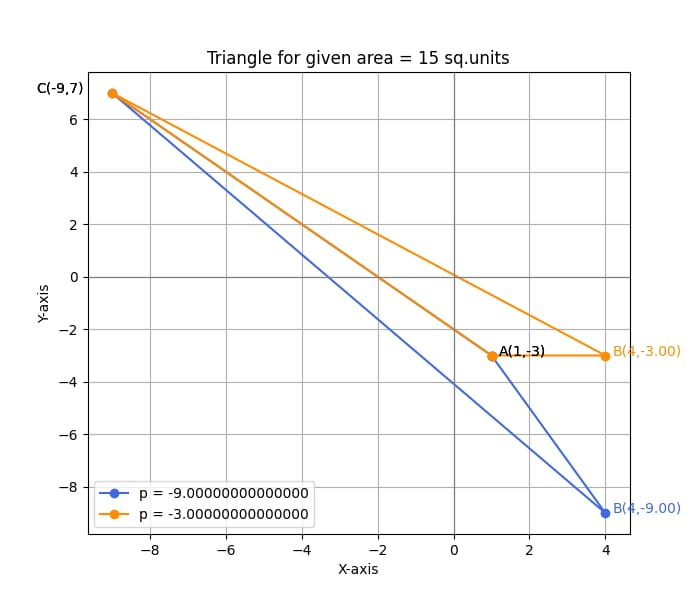
\includegraphics[width=0.75\columnwidth]{graph-1.png}
    \caption{Plot}
    \label{fig:placeholder}
\end{figure}


\end{document}